\section{Results}
\subsection{Calibration}

Due to small defects in the construction of the telescope and limitations of the motors of the dish and the antenna, the pointing of the antenna doesn't always line up with the target. It is therefore necessary to calibrate it before pointing at distant objects. The Sun is the strongest discrete radio source in the sky \cite{burke_introduction_2013}, mostly due to black body radiation, and is therefore an ideal target for the calibration.
By configuring the antenna to point towards Sun, using its actual coordinates, and scanning the surrounding area in Az/Alt coordinates, the maximum average measured power gives the real position of the Sun in the specific antenna coordinates. The measured power and a linear interpolation of those values shown in \autoref{fig:calibration_contour} gives a correction to the pointing of
\begin{equation} \label{eq:offset}
    \Delta a = -(5.25 \pm 0.50)^\circ \quad \textrm{and} \quad \Delta h = -(2.70 \pm 0.10)^\circ
\end{equation}
\begin{figure}[htbp]
    \centering
    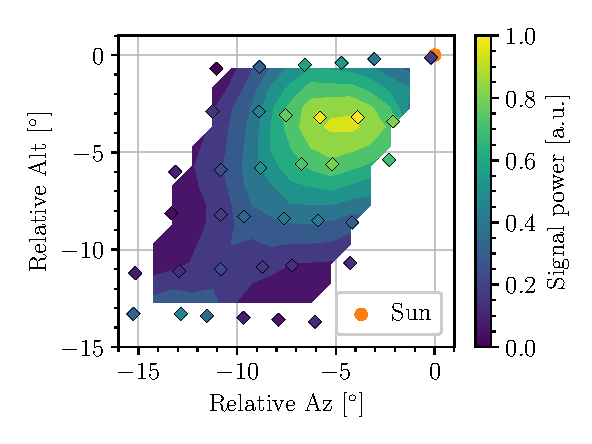
\includegraphics[scale=1]{figures/calibration_contour.pdf}
    \caption{Interpolation of signal power measured in the proximity of the Sun.}
    \label{fig:calibration_contour}
\end{figure}

\subsection{Distinguishing signal and noise}
The signal received by the antenna inherently contains noise which must be removed for the data to be properly analysed.
To this end, a signal measure was taken with the telescope pointed towards a nearby building, so that the registered spectrum  contained only the noise characteristic of the telescope location, which is expected to be found in all the signals received by the antenna.
The spectra of all the subsequently acquired signals were then divided by this noise spectrum, obtaining  signal-to-noise ratios which were further cleaned up by applying a moving average filter \hl{or median in some cases?}.
An example of the application of this pipeline is depicted in \autoref{fig:process_example}.
\begin{figure}
    \begin{subfigure}{0.49\textwidth}
        \centering
        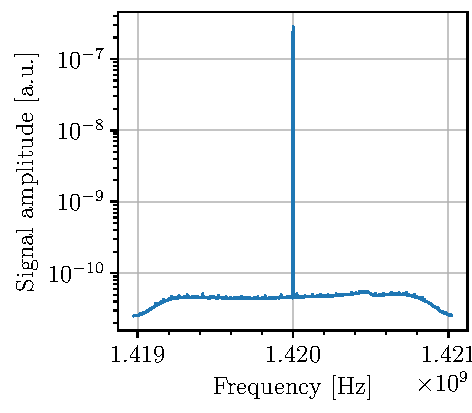
\includegraphics[scale=1]{figures/raw_signal.pdf}
        \caption{}
        \label{fig:raw_signal}
    \end{subfigure}
    \begin{subfigure}{0.49\textwidth}
        \centering
        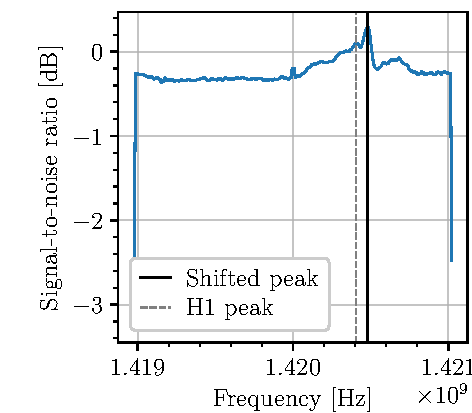
\includegraphics[scale=1]{figures/clean_signal.pdf}
        \caption{}
        \label{fig:clean_signal}
    \end{subfigure}
    \caption{Unprocessed and Processed}
    \label{fig:process_example}
\end{figure}


\subsection{Velocity curve of the Milky Way}
A series (\hl{different series?}) of spectra were acquired pointing VEGA to Galactic coordinates $b = 0$ and $3 \leq \ell \leq 160$ \hl{check valeurs exactes}, spanning almost half of the galactic plane.
Once the frequency shift of the hydrogen 21 cm line was identified in each spectra, \hl{the methods presented in the Theory or Annex} were used to derive the velocity of the hydrogen cloud observed, its distance from the Galactic Center and its distance from the Solar System.
\autoref{fig:VEGA_velocity_curve} depicts the velocity curves obtained using \hl{the different methods}.
\hl{Ici décrire les courbes et les differences obtenues avec les differentes methodes}.

By combining the distance of the hydrogen from Earth and the angle at which the measures were taken, a map of the Galaxy was produced as shown in \autoref{fig:VEGA_galaxy_map}. One can see how a spiral pattern was produced by the data.

À METTRE AVEC LES METHODES?: The movement of Earth inside the Solar System was neglected.

Talk about orientation (i.e. sky visible at measuring time)

\begin{figure}[htbp]
    \begin{minipage}[t]{0.5\textwidth}
        \centering
        \captionsetup{width=.9\textwidth}
        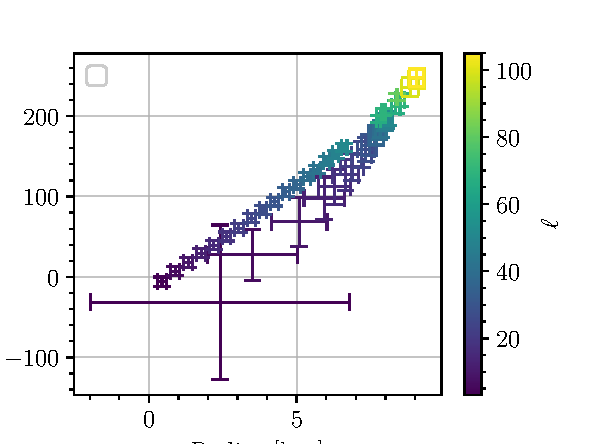
\includegraphics[scale=1]{figures/VEGA_velocity_curve.pdf}
        \caption{Velocity curve VEGA}
        \label{fig:VEGA_velocity_curve}
    \end{minipage}
    \begin{minipage}[t]{0.5\textwidth}
        \centering
        \captionsetup{width=.9\textwidth}
        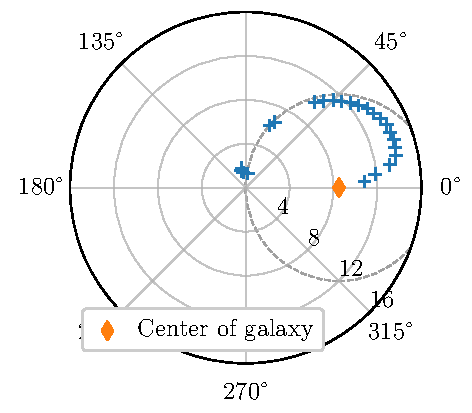
\includegraphics[scale=1]{figures/VEGA_galaxy_map.pdf}
        \caption{Galaxy map VEGA}
        \label{fig:VEGA_galaxy_map}
    \end{minipage}
\end{figure}

\subsection{Comparison with SALSA}
Since VEGA is very young, we wished to test the data analysis pipeline with a more mature telescope: one of the three SALSA (Such A Lovely Small Antenna) radio telescopes, based in Onsala Observatory, Sweden.
It is an antenna of similar size and conception and VEGA

Built-in correction for movement of Earth in solar system
\begin{figure}[htbp]
    \begin{minipage}[t]{0.5\textwidth}
        \centering
        \captionsetup{width=.9\textwidth}
        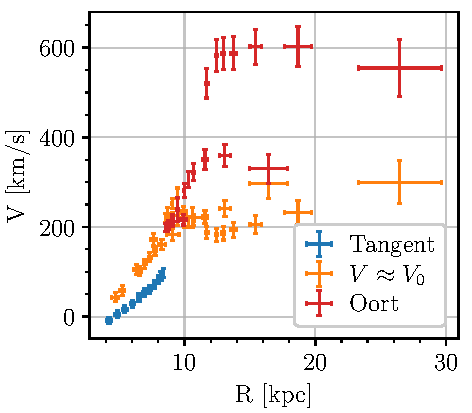
\includegraphics[scale=1]{figures/SALSA_velocity_curve.pdf}
        \caption{Velocity curve SALSA}
        \label{fig:SALSA_velocity_curve}
    \end{minipage}
    \begin{minipage}[t]{0.5\textwidth}
        \centering
        \captionsetup{width=.9\textwidth}
        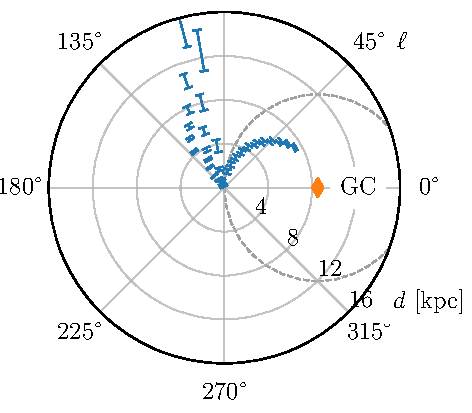
\includegraphics[scale=1]{figures/SALSA_galaxy_map.pdf}
        \caption{Galaxy map SALSA}
        \label{fig:SALSA_galaxy_map}
    \end{minipage}
\end{figure}